\chapter{Resultados}

Os resultados obtidos com as simulações estão descrito abaixo.

\section{Busca linear}

Na figura abaixo temos o resultado de .... Fazendo um ajuste dos pontos da curva conseguimos determinar que o comportamento é linear.


\begin{figure}[H]
  \centering
  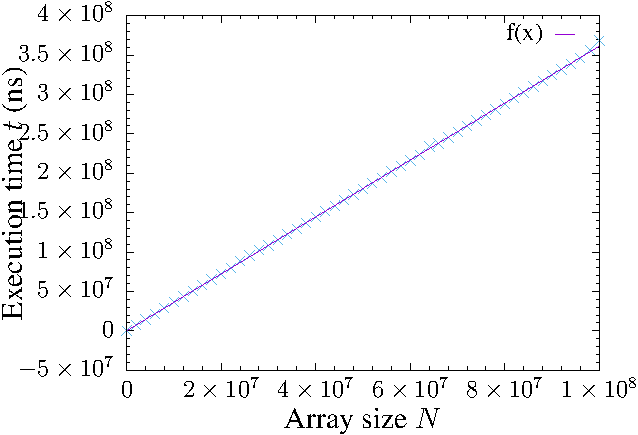
\includegraphics[scale=1.2]{../plots/lsearch_time.pdf}
  \caption{Tempo vs...}
\end{figure} \label{fig:lseach_time}


\section{Busca binária}

Na figura abaixo temos o resultado de .... Fazendo um ajuste dos pontos da curva conseguimos determinar que o comportamento é logarítmico.


\begin{figure}[H]
  \centering
  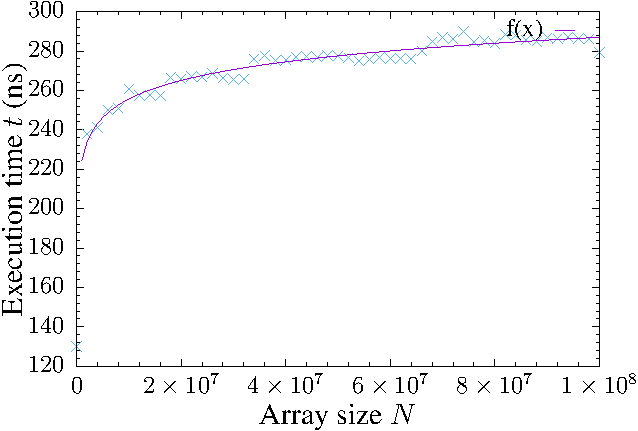
\includegraphics[scale=1.2]{../plots/bsearch_it_time.pdf}
  \caption{Tempo vs...}
\end{figure} \label{fig:bseach_it_time}

Na figura abaixo temos o resultado de .... Fazendo um ajuste dos pontos da curva conseguimos determinar que o comportamento é logarítmico.


\begin{figure}[H]
  \centering
  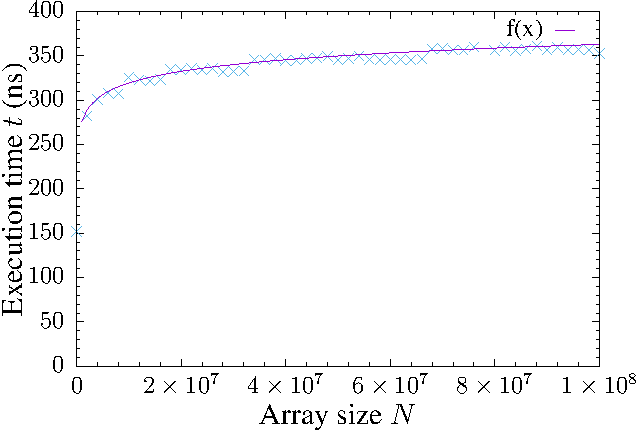
\includegraphics[scale=1.2]{../plots/bsearch_rec_time.pdf}
  \caption{Tempo vs...}
\end{figure} \label{fig:bseach_rec_time}


\section{Busca ternária}

Na figura abaixo temos o resultado de .... Fazendo um ajuste dos pontos da curva conseguimos determinar que o comportamento é logarítmico.


\begin{figure}[H]
  \centering
  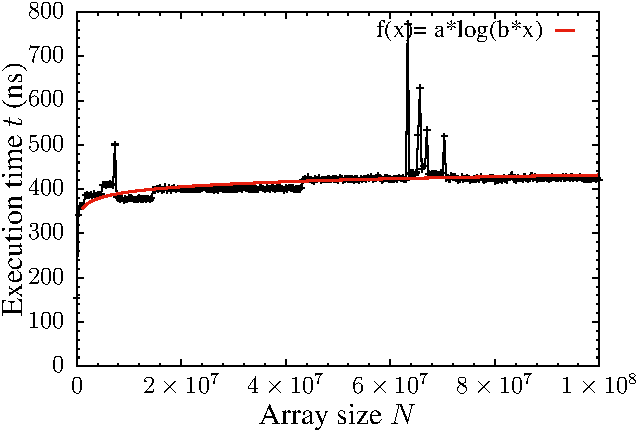
\includegraphics[scale=1.2]{../plots/tsearch_it_time.pdf}
  \caption{Tempo vs...}
\end{figure} \label{fig:tseach_it_time}

Na figura abaixo temos o resultado de .... Fazendo um ajuste dos pontos da curva conseguimos determinar que o comportamento é logarítmico.


\begin{figure}[H]
  \centering
  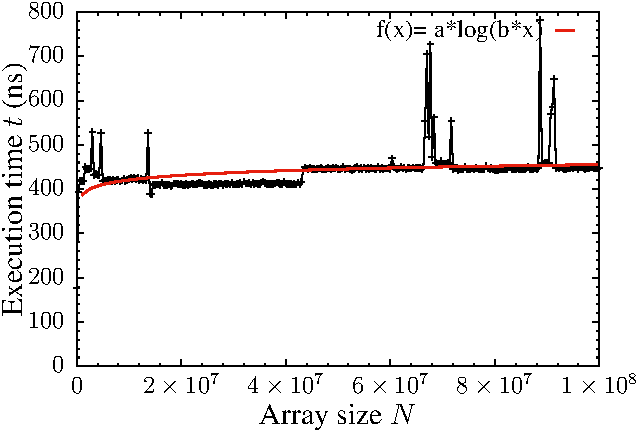
\includegraphics[scale=1.2]{../plots/tsearch_rec_time.pdf}
  \caption{Tempo vs...}
\end{figure} \label{fig:tseach_rec_time}

\section{{\it Jump search}}

Na figura abaixo temos o resultado de .... Fazendo um ajuste dos pontos da curva conseguimos determinar que o comportamento se aproxima de um comportamento quadrático.


\begin{figure}[H]
  \centering
  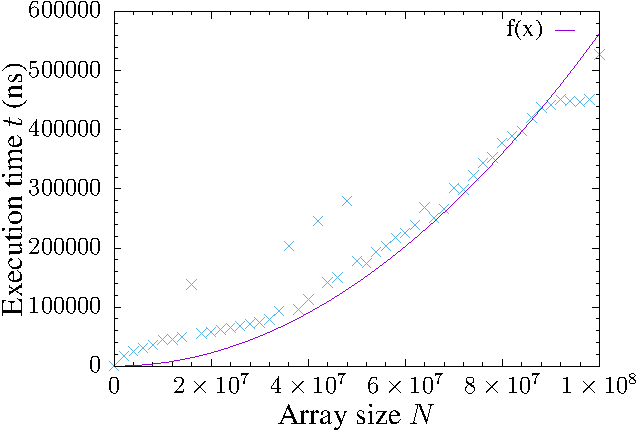
\includegraphics[scale=1.2]{../plots/jumpsearch_time.pdf}
  \caption{Tempo vs...}
\end{figure} \label{fig:jumpsearch_time}

\section{Busca de Fibonacci}
